\chapter{Ordinary Differential Equations}
\section{Definition and Terminology} \label{def-de}
We shall classfy differential equations according to 
\textbf{type, order and linearity}

\begin{itemize}
    \item[Types]
        \begin{itemize}
            \item ODE\footnote{Only the ODE is required by NUGEE.}
            \item PDE
        \end{itemize}
    \item[Order]
        The meaning of \textbf{order} is same as the 
        \textbf{order} of differentiation.
    \item[Linearities]
        The meaning of \textbf{degree} is same as the 
        the \textbf{degree} of polynomial.
\end{itemize}

\subsection{Verification of Solutions}

A solution of a differnential equation that is identically zero
on an interval $I$ is said to be a \textbf{trivial solution}.

You have to check the solution of a differential equation wether
or not fit it's interval of definition (domain).

\subsection{Function v.s. Solution}

You have to check the solution of a differential equation wether
or not fit it's interval of definition (domain).

The domain of $y = 1/x$, considered simply as a \textbf{function}, 
is the set of all real numbers $x$ except $0$. 

Now $y = 1/x$ is also a \textbf{solution} 
of the linear first-order differential equation
$xy' + y = 0$. (Verify.) But when we say that $y = 1/x$ 
is a \textbf{solution of this DE}, we
mean that it is a function defined 
\emph{on an interval I} on which it is differentiable and
\emph{satisfies} the equation\cite{fcde}.

\section{First-Order Differential Equations}

The \textbf{critical point} of a autonomous differential equation
is a constant number which satisfy $f(c) = 0$.
Meanwhile, $y(x) = c$ is also a constant solution of the equation.

A critical point is also called \textbf{equilibrium point} or
\textbf{stationary point}.

A constant solution $y(x) = c$ is called an 
\textbf{equilibrium solution}\cite{fcde}.

\subsection{Conclusions of Non-constant Solution of A Autonomous}

\begin{definition}
    [Autonomous differential equation] is a First-Order Differential Equations which like
    \[
        \dfrac{\mathrm{d}y}{\mathrm{d}t} = f(y)
    \]

    Many differential equations encountered in applications or equations that are
    models of physical \emph{laws that do not change over time} are autonomous\cite{fcde}.
\end{definition}

\begin{itemize}
    \item Non-constant solution do not cross the equilibrium solution.
    \item $f(y)$ do not change the signs in a subregion.
    \item a solution $y(x)$ is strictly monotonic in s subregion.
    \item If $y(x)$ is \emph{bounded}
        \begin{itemize}
            \item[above] by a critical point $c_1$,
                then the graph of $y(x)$ must approach the graph of the
                equilibrium solution $y(x) = c_1$ 
                either as $x \to \infty$ or as $x \to - \infty$.
            \item[(both)] by two consecutive critical points 
                $c_1$ and $c_2$ (as in subregion where $c_1 < y(x) < c_2$ for all $x$),
                then the graph of $y(x)$ must approach the graph of the
                equilibrium solutions $y(x) = c_1$ and $y(x) = c_2$
                one as $x \to \infty$, the other as $x \to - \infty$.
            \item[below] by a critical point $c_2$,
                then the graph of $y(x)$ must approach the graph of the
                equilibrium solution $y(x) = c_2$ 
                either as $x \to \infty$ or as $x \to - \infty$.
        \end{itemize}
\end{itemize}

\subsection{Solution Curves of an Autonomous DE}

\begin{example}
    \[
        \dfrac{\mathrm{d}y}{\mathrm{d}x} = \sin y
    \]

    \begin{verbatim}
StreamPlot[
    {1, Sin[y]}, 
    {x, -2, 2}, {y, -2 Pi, 2 Pi}
]
    \end{verbatim}
    \begin{figure}[H]
        \centering
        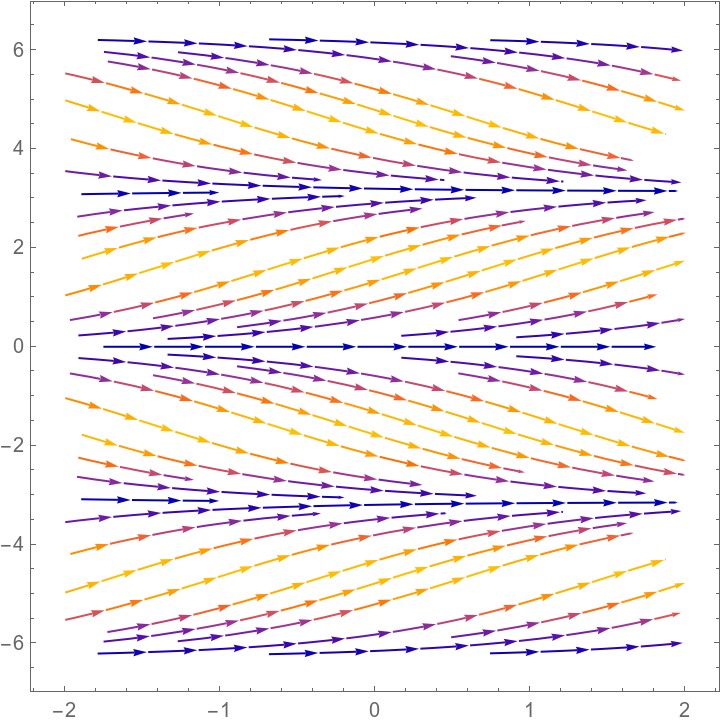
\includegraphics[width = \textwidth]{figure/direction-field-dy-slash-dx-siny}
        \caption{the direction field of $dy/dx = \sin y$}
        \label{fig:direction-field-dy-slash-dx-siny}
    \end{figure}
\end{example}

By the figure \ref{fig:direction-field-dy-slash-dx-siny}, we know
the slopes of lineal elements on a horizontal line are all the same.

Thus we could got 
\begin{corollary}[The Transltion Property of autonomous DEs]
    If $y(x)$ is a solution of an autonomous differential equation
    $dy/dx = f(y)$, then $y_1(x) = y(x - k)$, $k$ a constant,
    is also a solution.
\end{corollary}

\subsection{Solutions of Separable Equations}
\label{solutions-of-separable-equations}

\begin{definition}
    A first-order differential equation of the form
    \begin{equation}\label{eq:form-of-separable-equation}
        \dfrac{\mathrm{d}y}{\mathrm{d}x} = g(x)h(y)
    \end{equation}
    is said to be separable or to have separable variables.
\end{definition}

You basically convert the euqation \ref{eq:form-of-separable-equation} into
\begin{align*}
    1/h(y) \mathrm{d}y &= g(x) \mathrm{d}x\\
    \int 1/h(y) \mathrm{d}y &= \int g(x) \mathrm{d}x
\end{align*}
after that, you could get the solution(s).

Sometime, the antiderivatives of each side could not be 
representde by a elementary function. 
In this case, the solutions could only be represented by a 
integral-defined function
\[
    y(x) = y_0 + \int_{x_0}^{x} g(t) \mathrm{d}t
\]

\subsection{Solutions of a Linear First-Order DE}

\begin{enumerate}
    \item Remember to put a linear equation into the standard form
        \begin{equation}\label{eq:standard-form-of-linear-ODE}
            \dfrac{\mathrm{d}y}{\mathrm{d}x} + P(x) y = f(x)
        \end{equation}
        both the coefficient function $P(x)$ and $f(x)$
        \textbf{are continuous on the interval $I$}.
    \item 
        From the standard form of the equation 
        identify $P(x)$ and then find the
        integrating factor
        $e^{\int P(x) \mathrm{d}x}$
        . 
        No constant need be used in evaluating the
        indefinite integral $\int P(x) \mathrm{d}x$.
    \item 
        Multiply the both sides of the standard form equation by the integrating
        factor. The left-hand side of the resulting equation 
        is automatically\footnote{See also \cite[page 55]{fcde}} the
        derivative of the product of the integrating factor
        $\cramped{e^{\int P(x) \mathrm{d}x}}$
        and $y$:
        \begin{equation}
            \dfrac{\mathrm{d}}{\mathrm{d}x}
            \left[
                e^{\int P(x) \mathrm{d}x} y
            \right]
            =
            e^{\int P(x) \mathrm{d}x} f(x)
        \end{equation}
    \item 
        Integrate both sides of the last equation and solve for $y$\cite[page 56]{fcde}.
        \begin{gather}\label{eq:solution-linear-first-order-DE}
            \int
                \dfrac{\mathrm{d}}{\mathrm{d}x}
                \left[
                    e^{\int P(x) \mathrm{d}x} y
                \right]
            \mathrm{d}x
            = \int e^{\int P(x) \mathrm{d}x} f(x) \mathrm{d}x \notag \\
            y = e^{-\int P(x) \mathrm{d}x} 
            \left[
                \int f(x) e^{\int P(x) \mathrm{d}x} \mathrm{d}x + C
            \right]
        \end{gather}
        See also \cite[page 139, pdf 150]{we}.
\end{enumerate}

Function
\[
    \mu (x) = e^{\int P(x) \mathrm{d}x}
\]
is called \textbf{integrating factor} for equation \ref{eq:standard-form-of-linear-ODE}.

\begin{example}
    IVP:
    \[
        y \dfrac{\mathrm{d}x}{\mathrm{d}y} -x = 2y^2, \quad y(1) = 5.
    \]
    \cite[page 63]{fcde}

\end{example}

\section{Exact Equations}

\begin{definition}[Exact Equation] \label{def:exact-equation}
    A differential expression $M(x, y) \mathrm{d}x + N(x, y) \mathrm{d}y$
    is an \textbf{exact differential} in a region $R$ of the 
    xy-plane if it corresponds to the differential of some function
    $f (x, y)$ defined in $R$. 
    A first-order differential equation of the form
    \[
        M(x, y) \mathrm{d}x + N(x, y) \mathrm{d}y = 0
    \]
    is said to be an 
    \textbf{
        exact
        \footnote{
            An equation is called \emph{exact}
            when it can be expressed as 
            the derivative of a function 
            (often referred to as a potential function 
            or a primitive function). 
            In other words, equations satisfied \ref{eq:criterion-for-an-exact-differential}
            would be called exact.
        } equation
    } if the expression on the 
    LHS is an exact differential.
    \cite[page 65]{fcde}
\end{definition}

Once we get the \emph{exact equation}, 
we could get the implicit solution(s)
via some way.

\begin{theorem}[Criterion for an Exact Differential]
    \label{criterion-for-an-exact-differential}
    Let $M(x, y)$ and $N(x, y)$ be continuous and 
    have continuous first partial derivatives 
    in a rectangular region $R$ defined by $a < x < b, c < y < d$. 
    Then a necessary and sufficient condition that 
    $M(x, y) \mathrm{d}x + N(x, y) \mathrm{d}y$ be an exact
    differential is
    \begin{equation}\label{eq:criterion-for-an-exact-differential}
        \dfrac{\partial M}{\partial y} = \dfrac{\partial^2 f}{\partial y \partial x} = \dfrac{\partial N}{\partial x}  
    \end{equation}
\end{theorem}
 
The equality of the mixed partials is a consequence of 
the \textbf{continuity} of the first partial derivatives of 
\[
    M(x, y) \quad \mbox{and} \quad N(x, y).
\]

The sufficiency part of Theorem \ref{criterion-for-an-exact-differential} 
consists of showing that there exists a function $f$ for which
\[\partial f/ \partial x = M(x, y)\] and \[\partial f/ \partial y = N(x, y)\]
when ever (\ref{eq:criterion-for-an-exact-differential}) holds.
The construction of the function $f$ actually reflects a basic procedure
for solving exact equations,

In other words:
\[
    \dfrac{\partial M}{\partial y} = \dfrac{\partial N}{\partial x}  
    \Longrightarrow 
    \dfrac{\partial f}{\partial x} = M(x, y) 
    \bigwedge
    \dfrac{\partial f}{\partial y} = N(x, y) 
\]

We can find $f$ by integrating $M(x, y)$ 
with respect to $x$ while holding $y$ constant:
\[
    f(x, y) = \int M(x, y) \mathrm{d}x + g(y)
\]
where the arbitrary function $g(y)$ is the \emph{constant} of integration. 

After that, 
\[
    \dfrac{\partial f}{\partial y} = \dfrac{\partial}{\partial y}
    \int M(x, y) \mathrm{d}x + g'(y) = N(x, y)
\]
then you can get the $g'(x)$, moreover by integrading $g(y)$ also got.

\begin{example}
    IVP:
    \[
        \dfrac{\mathrm{d}y}{\mathrm{d}x} = 
        \dfrac{xy^2 - \cos x \sin x}{y(1-x^2)}, \quad y(0) = 2.
    \]
    \cite[page 68]{fcde}
\end{example}

\subsection{Integrading Factor}

Multiplying a \textbf{integrading factor} on both side of a nonexact equation
\[
    \mu (x, y) M(x, y) \mathrm{d}x + \mu (x, y) N(x, y) \mathrm{d}y = 0
\]
could convert it into a exact equation.

See also \cite[page 68]{fcde}.

\section{High-Order Differential Equations}

\subsection{Reduction of Order} \label{reduction-of-order}

\begin{enumerate}
    \item Put equation
        \[
            a_2(x)y'' + a_1(x) y' + a_0(x) y = 0
        \]
        into 
        \begin{equation}\label{eq:standard-form-linear-DE-2}
            y'' + P(x)y'x + Q(x)y = 0
        \end{equation}
        where $P$ and $Q$ are continuous on some interval $I$.
    \item Suppose $y_1$ is a konwn solution of \ref{eq:standard-form-linear-DE-2} on $I$
        and that $y_1(x) \neq 0$ for every $x$ in the interval.
        if we \textbf{define} $y = u(x)y_1(x)$, it follows that
        \begin{align}
            y'  &= u y'_1 + y_1 u' \notag\\
            y'' &= uy''_1 + 2y_1'u' + y_1 u'' \notag\\
            y'' + Py'x + Qy &= 
                u\underbrace{
                    \left[y_1'' + Py_1' + Qy_1\right]
                }_{\mathclap{
                    =0 \mbox{, \,= equation \ref{eq:standard-form-linear-DE-2}}
                }}\notag\\
                &+ y_1u'' + (2y_1' + Py_1) u' = 0 \label{eq:before-rename-of-linear-ODE-when-reduction-order}
        \end{align}
    \item Let $w = u'$, thus equation \ref{eq:before-rename-of-linear-ODE-when-reduction-order} turns into
        \[
            y_1w' + (2y_1' + Py_1) w = 0
        \]
    \item By separating variables and integrating, we obtain
        \begin{equation}\label{eq:another-sln-reduction-order}
            y_2 = y_1(x) \int \dfrac{e^{-\int P(x) \mathrm{d}x}}{{y_1}^2 (x)} \mathrm{d}X
        \end{equation}
\end{enumerate}

\subsection{Homogeneous Linear Equations with Constant Coefficients}
\label{homogeneous-linear-equations-with-constant-coefficients}

\begin{example} \label{ex:introductory-example-one-order-homo-linear-DE}
    Solving $ay' + by = 0$ for $y'$ yields $y' = ky$, 
    where $k$ is a constant. This observation reveals
    the nature of the unknown solution $y$.

    \emph{The only nontrivial elementary function whose
    derivative is a constant multiple of itself is 
    an exponential function} $e^{mx}$.

    If we substitute $y = e^{mx}$ and $y' = me^{mx}$ into $ay' + by = 0$, 
    we get
    \[
        ame^{mx} + be^{mx} = 0 \quad \mbox{or} \quad e^{mx}(am + b) = 0
    \]
    Since $e^{mx}$ is never zero for real number $x$, that's impiles
    \begin{equation}\label{eq:a-simple-example-of-aux-equation}
        am + b = 0
    \end{equation}
    For this single value of $m$, $y = e^{mx}$ is a solution of the DE.
    Equation \ref{eq:a-simple-example-of-aux-equation} is called \textbf{auxiliary equation}.
\end{example}

The foregoing procedure can produce exponential solutions
for homogeneous linear higher-order DEs.
\begin{equation}\label{eq:standard-form-high-order-homogeneous-linear-DE}
    y^{(n)} + a_{n-1}y^{(n-1)} + \ldots + a_1y' + a_0y = 0
\end{equation}
where the Coefficients $a_i, i = 0, 1, \cdots, n$ are real constants
and $a_n \neq 0$.

For 2-order HLDEs, we have auxiliary equation
\[
    am^2 + bm + c = 0
\]

There're 3 types of solution which we can use:
\begin{itemize}
    \item[$\Delta > 0$] We could get two solutions: 
        \[
            y_1 = e^{m_1x} \quad \mbox{and} \quad y_2 = e^{m_2x}
        \]
    \item[$\Delta = 0$] We could get one solution directly: $y_1 = e^{m_1x}$.
        The other solution could be solved by the equation 
        \ref{eq:another-sln-reduction-order}
        \begin{align}\label{eq:complementary-func-sln-delta-0}
            y_2 &= e^{m_1 x} \int \dfrac{e^{2 m_1 x}}{e^{2 m_1 x}} \mathrm{d}x = e^{m_1 x} \int \mathrm{d}x \notag \\
                &= x e^{m_1 x}
        \end{align}
    \item[$\Delta < 0$]
        If $m_1$ and $m_2$ are complex, then we can write
        \[
            m_1 = \alpha + i \beta \quad \mbox{and} \quad m_2 = \alpha - i \beta
        \]
        the general solution is
        \begin{equation}
            y(x) = e^{\alpha x}(c_1 \cos(\beta x) + c_2 \sin(\beta x))
        \end{equation}
\end{itemize}

\subsection{Non-homogeneous DE with Undertermined Coefficients - Superposition Approach}

\begin{definition}[Standard Form of Non-homogeneous Linear Differential Equation]
    \label{def:non-homo-linear-DE}
    \begin{equation}\label{eq:standard-form-non-homogeneous-linear-DE}
        y^{(n)} + a_{n-1}y^{(n-1)} + \ldots + a_1y' + a_0y = g(x)
    \end{equation}
    $g(x)$ is a linear combination of elementary functions.
    The equation is a \emph{homogeneous DE} 
    when $g(x) = 0$.
\end{definition}

\begin{theorem}[General Solution - Non-homogeneous Differential Equations]
    \label{general-sln-non-homo-DE}
    Let $y_p$  be any particular solution of 
    the nonhomogeneous linear $n$th-order
    differential equation \ref{eq:standard-form-non-homogeneous-linear-DE}
    on an interval $I$, 
    and let $y_1, y_2, \cdots, y_n$ be a fundamental set of 
    solutions of the associated homogeneous differential equation
    \footnote{
        which $g(x)$ in equation 
        \ref{eq:standard-form-non-homogeneous-linear-DE} 
        is identically zero.
    }
    on $I$.
    Then the general solution of the equation on the interval is
    \[
        y = 
        \underbrace{
            c_1 y_1(x) +
            c_2 y_2(x) +
            \cdots
            c_n y_n(x) 
        }_{\mathclap{\mbox{
            Complementary function
        }}}
        + y_p(x)
    \]
    where the $\cramped{c_i}, i = 1, 2, \cdots, n$ are arbitrary constants.
\end{theorem}
By the way, there's no any constant coeffient beside 
the particular term\footnote{namely, $y_p$.}.

Way to solve it:
\begin{enumerate}
    \item Find the complementary function $y_c$, and 
    \item find \emph{any} particular solution $y_p$ of 
        the nonhomogeneous equation 
        \ref{eq:standard-form-non-homogeneous-linear-DE}.
\end{enumerate}
We could determine the form of 
the particular function by the form of $g(x)$.
See also table \ref{tab:useful-form-map-y_p-gx}.

\begin{table}[b]
    \centering
    \begin{tabular}{cl}
        \toprule
        $g(x)$ & Form of $y_p$ \\
        \midrule
        $\cramped{1              }$ & $\cramped{A                                                }$\\
        $\cramped{5x + 7         }$ & $\cramped{Ax + B                                           }$\\
        $\cramped{3x^2 - 2       }$ & $\cramped{Ax^2 + Bx + C                                    }$\\
        $\cramped{x^3 -x + 1     }$ & $\cramped{Ax^3 + Bx^2 + Cx + E                             }$\\
        $\cramped{\sin 4x        }$ & $\cramped{A\cos 4x + B \sin 4x                             }$\\
        $\cramped{\cos 4x        }$ & $\cramped{A\cos 4x + B \sin 4x                             }$\\
        $\cramped{e^{5x}         }$ & $\cramped{Ae^{5x}                                          }$\\
        $\cramped{(9x - 2)e^{5x} }$ & $\cramped{(Ax + B) e^{5x}                                  }$\\
        $\cramped{xe^{3x} \cos 4x}$ & $\cramped{(Ax + B) e^{3x} \cos 4x + (Cx + E)e^{3x}  \sin 4x}$\\ 
        \bottomrule
    \end{tabular}
    \caption{$g(x)$, RHS of a linear nonhomogeneous DE, and corresponding forms of the particular solution}
    \label{tab:useful-form-map-y_p-gx}
\end{table}

\begin{example}
    Find a particular solution of
    \[
        y'' - 2y' -3 y = 4x - 5 + 6x e^{2x}
    \]

    \begin{itemize}
        \item The complementary function is
            \[
                y_c = c_1 e^{-x} + c_2 x e^{3x}
            \]
        \item By the table \ref{tab:useful-form-map-y_p-gx}, we guess a particular function is
            \[
                y_p = Ax + B + Cx e^{2x} + E e^{2x}
            \]
            Substituting it into the given equation and grouping like terms gives
            \begin{align*}
                  &y''_p - 2y'_p - 3y_p  \\
                = &\underbrace{-3A}_{4}x \underbrace{-2A -3B}_{-5} \underbrace{-3C}_{6} xe^{2x} + \underbrace{(2C - 3E)}_{0} e^{2x}\\
                = &4x - 5 + 6x e^{2x}
            \end{align*}
        \item Consequently,
            \begin{align*}
                y &= c_1 e^{-x} + c_2 x e^{3x}\\ 
                  &- \dfrac{4}{3} x + \dfrac{23}{9} - \left(2x + \dfrac{4}{3}\right) e^{2x}
            \end{align*}
    \end{itemize}
\end{example}

\subsection{A Glich in the Method}\label{glich-in-superposition-method}

But there're possibly some terms exist which repeated in both the complementary and particular function.
For example:
\begin{equation}\label{eq:example-non-homo-DE}
    y'' - 5y' + 4y = 8 e^x 
\end{equation}
\begin{align}
    y_c &= c_1 e^x + c_2 e^{4x} \notag\\
    y_p &= A e^x \quad  \mbox{(impropriate)} \label{eq:impropriate-guessed-particular-function-form}
\end{align}
Observe that our assumption $Ae^x$ is already present in $y_c$. This
means that $e^x$ is a solution of the associated 
homogeneous differential equation, and
a constant multiple $Ae^x$ when substituted into the 
differential equation necessarily
\emph{produces zero}\cite[page 146]{fcde}.

Inspired by the equation \ref{eq:complementary-func-sln-delta-0}, 
we could just multiply a $x$ at \ref{eq:impropriate-guessed-particular-function-form}.
now
\[
    y_p = Ax e^x
\]
and by substituting $y_p$ into the DE, we get
\[
    y''_p - 5 y'_p + 4y_p = -3A e^x = 8e^x
\]

By the way, only the duplicated terms need to be multiplied a $x$ factor,
others can't. See also \cite[page 145, pdf 156, example 3]{we}.
\begin{example}
    DE
    \[
        y'' - y = e^x + 1
    \]
    What is the particular function assumption could be? 

    Solution:
    \[
        y_p = Axe^x + B
    \]
    Consequently,
    \[
        y''_p - y_p = 2Ae^x - B
    \]

    If you let
    \[
        y_p = Axe^x + Bx\quad \mbox{(impropriate)}
    \]
    Consequently,
    \[
        y''_p - y_p = 2Ae^x - Bx
    \]
\end{example}

See also exmaple 8 \cite[page 148]{fcde}.

\section{考点补充}

微分方程相关题目有下面几个考察方式:
\begin{itemize}
    \item 计算 
    \item 综合题(难点)
    \item 应用题
\end{itemize}

其中,Homogeneous Linear Equations with Constant Coefficients 是考察的重点。
参见小节 \ref{homogeneous-linear-equations-with-constant-coefficients}。

\subsection{计算}

\begin{example}
    \[
        y' = \dfrac{1}{xy + y^3}
    \]
    \cite[page 143, pdf 154]{we}.

    \begin{align*}
        \dfrac{\mathrm{d}y}{\mathrm{d}x} = \dfrac{1}{xy + y^3}
    \end{align*}
    看到这里,题目似乎并不是我们了解的类型。
    但是请注意,\textbf{导数是微分的商}。因此,我们可以对调微分的位置,则
    \[
        \dfrac{\mathrm{d}x}{\mathrm{d}y} = {xy + y^3}
    \]
    现在的未知函数变为了 $x(y)$. 

    将式子化为标准形式\footnote{公式 \ref{eq:standard-form-of-linear-ODE}}后,
    利用公式 \ref{eq:solution-linear-first-order-DE} 求出
    \[
        x = C e^{(1/2) y^2} - y^2 - 2
    \]

    最后结果就这样写即可,不用转化为 $y(x)$。

    \begin{equation*}
        \dfrac{\mathrm{d}x}{\mathrm{d}y} - yx = y^3
    \end{equation*}
    \begin{align*}
         &\int {P(y)} \mathrm dy = \int {-y} \mathrm dy = -\frac{y^2}{2}\\
        =&\int f(y) e^{\int P(y) \mathrm dy} \mathrm dy \\
        =&\int y^3 e^{-\frac{y^2}{2}} \mathrm dy = -\int y^2 \mathrm d e^{-\frac{y^2}{2}} \\
        =&-\left(y^2 e^{-y^2/2} - \int e^{-y^2/2} \mathrm dy^2\right)\\
        =&-\left(y^2 e^{-y^2/2} - \int 2y e^{-y^2/2} \mathrm dy\right)\\
        =&-\left(y^2 e^{-y^2/2} + \int 2 \mathrm de^{-y^2/2}\right)\\
        =&-\left(y^2 e^{-y^2/2} + 2\int \mathrm de^{-y^2/2}\right)\\
        =&-\left(y^2 e^{-y^2/2} + 2e^{-y^2/2}\right)\\
        =&-e^{-\frac{y^2}{2}} (2 + y^2)\\
        x=&e^{-\int P(y) \mathrm dy} \left[\int f(y) e^{\int P(y) \mathrm dy} \mathrm dy + C\right] \\
        =&e^{y^2/2} \left[-e^{-y^2/2}\left(2+y^2\right) + C\right] \\
        =& C e^{(1/2) y^2} - y^2 - 2
    \end{align*}
    分部积分请参见 \ref{part-integral}
\end{example}

\begin{example}
    \[
        y' = \cos (x+y)
    \]
    该题目进行变量对调(微分)也没用,则还可以考虑\textbf{变量代换}。

    令
    \begin{gather*}
        u  = x+ y \\
        y' = u' - 1 = \cos u\\
        \frac{\mathrm du}{\mathrm dx} = 1+ \cos u \\
        \int \frac{\mathrm du}{1+\cos x} = \int \mathrm dx 
    \end{gather*}
    则,原方程变化为 Separable DE
    \footnote{参见\ref{solutions-of-separable-equations}}.

    和上一个例子不同的是,本例最终结果要将 $u$ 还原为 $x+y$, 即
    \begin{align*}
        &\int \frac{\mathrm du}{1+\cos u} =\int \frac{\mathrm du}{2 \cos^2 \frac{u}{2}} \quad \mbox{\small (推论 \ref{co:trig-order-raising-equations})}\\
        =&\int \frac{1}{2} \sec^2 \frac{u}{2} \mathrm du =\tan \frac{u}{2} + C\\
        \Rightarrow &\tan \dfrac{x+y}{2} = x + C
    \end{align*}
\end{example}

综上两个例子,遇到需要变形才能进一步分类的微分方程求解问题,有下面两个主要方法:
\begin{itemize}
    \item 变量对调(微分)
    \item 变量代换
\end{itemize}

\subsection{综合题 - 用特征方程推出方程}

本方法需要通过齐次的两个线性无关解找出特征方程,
进而通过特征方程推导出微分方程。
这里面,关键在于如何通过非齐次的一个解找出其他两个齐次的解。

\begin{example}
    若 
    \begin{align}
        \notag y &= e^{2x} + (x+1) e^x \\
        \label{eq:expanded-form-a-complex-example-1} &= e^{2x} + x e^x + e^x \\
        \notag   &= y_c + y_p
    \end{align}
    是方程 
    \[
        y'' + ay' + by = ce^{x}
    \]
    的解,求 $a, b, c$ 以及该方程通解。

    \cite[page 145, pdf 156]{we}
    
    通过原方程的RHS可知,
    \[
        y_p = Ae^{m_1x} 
        \quad \mbox{or} \quad 
        y_p = Axe^{m_2x} \mbox{(impropriate)}
    \]
    因此解中的 $\cramped{e^{2x}}$ 必为一个$y_c$ 
    那么特征方程必有必有一解为 $2$, 即$m_1 = 2$.
    另一个特解$y_p$ 不能为
    \footnote{
        式子 (\ref{eq:expanded-form-a-complex-example-1}) 
        中的项 $\cramped{xe^x}$ ($A = 1$) 与之对应。
        既然不能是项 $xe^x$,那么就只能是 项$e^x$ 了,
        $\cramped{e^x = e^{m_2x} \Rightarrow m_2 = 1}$
    }
    $\cramped{Axe^x}$,
    这种情况
    \footnote{
        参见式子
        \ref{eq:complementary-func-sln-delta-0}
        和小节
        \ref{glich-in-superposition-method}
    }
    出现说明 $\Delta = 0$,
    即 $m_1 = m_2 = 1$,
    而事实上$m_1 = 2$.
    综上可列出特征方程
    \footnote{
        下面方程中,等号左边的因子 $(m - 1)$ 
        是基于对 $m_2 = 1$ 的推断。
        这一推断请参见第一条脚注
    }
    \begin{align*}
        (m-1)(m-2) &= 0\\
        m^2 - 3m + 2 &= 0
    \end{align*}
    则 $a = -3, b = 2$.

    将 $y = xe^x$ 带入方程 $y'' - 3y' + 2y = ce^x$ 得 $c = -1$,
    则所求方程通解为
    \[
        y = C_1 e^x + C_2 e^{2x} + xe^x
    \]
\end{example}
该例子用一句话概括就是通过已有信息将 $y$ 分为 $y_c$ 和 $y_p$
进而通过$y_c$找到特征方程。

\subsubsection{Non-homogeneous linear DE 解的性质补充}

请参见非齐次线性微分方程通解定理\ref{general-sln-non-homo-DE}。
可以看到项 $y_p$ 前是没有参数的。则对同一个微分方程的不同特解
\footnote{通解中取不同常数得到的解},
即便取的参数不同,他们中也必有相同的成分,也就是
$y_p$.

这样我们可得到下面的有用性质:
\begin{equation}
    y_1 - y_2 = y_c + (y_p - y_p) = y_c
\end{equation}
这条性质在没有提供微分方程,但是提供了它的几个特解时非常有用。
可以帮助我们找到特征方程。
另外,找到方程对应齐次解后,将题目给出的非齐解带入方程求出
\footnote{定义\ref{def:non-homo-linear-DE}}
$g(x)$ 写答案即可。

\begin{example}
    已知 $y_1 = 3, y_2 = 3 + x^2, y_3 = 3 + e^x$
    是某\uline{二阶线性非齐次}\footnote{注意了,没说是常系数}
    方程的三个特解。求该方程及通解。

    \cite[page 145, pdf 156, example 3(7)]{we}。

    \begin{align*}
        y_2 - y_1 &= x^2 \\
        y_3 - y_1 &= e^x 
    \end{align*}
    为齐次方程的两个线性无关特解,则所求方程的通解为
    \begin{align}
        \label{eq:general-sln-of-a-complex-example-1} y  &= C_1 e^x + C_2 e^{2x} + xe^x  \\
        \label{eq:general-sln-of-a-complex-example-2} y' &= 2C_1 x + C_2 e^x \\
        \label{eq:general-sln-of-a-complex-example-3} y''&= 2C_1 + C_2 e^x 
    \end{align}
    
    式 (\ref{eq:general-sln-of-a-complex-example-3}) 减 (\ref{eq:general-sln-of-a-complex-example-2}) 得
    \begin{equation}
        \label{eq:general-sln-of-a-complex-example-4}
        y'' - y' = C_1(1-x)
    \end{equation}
    式 (\ref{eq:general-sln-of-a-complex-example-1}) 减 (\ref{eq:general-sln-of-a-complex-example-2}) 得
    \begin{equation}
        \label{eq:general-sln-of-a-complex-example-5}
        y - y' = C_1(x^2 - 2x) + 3
    \end{equation}
    联立式子 (\ref{eq:general-sln-of-a-complex-example-4}) 和 (\ref{eq:general-sln-of-a-complex-example-5}) 可得
    \[
        (2x - x^2) y'' + (x^2 - 2) y' + 2(1-x)y = 6(1-x)
    \]
\end{example}

\subsubsection{错题收录}

有关降阶法其他内容请参见\ref{reduction-of-order}。

\begin{example}
    设 $a > 0$ 是常数,连续函数 $f(x)$ 满足 
    \[
        \lim_{x \to +\infty} f(x) = b
    \]
    $y = y(x)$ 是微分方程
    \[
        y'' + ay' = f(x) \quad \left(x \in [0, +\infty)\right) 
    \]
    的解,则求 $\lim_{x \to +\infty} y'(x), \lim_{x \to +\infty} y''(x)$ 

    \cite[question 77]{w660}.

    令 $p = y'$ 则原方程化为
    \[
        p' + ap = f(x)
    \]
    则由公式 (\ref{eq:solution-linear-first-order-DE}) 可得
    \[
        p = e^{-ax} \left[\int_0^x e^{ax} f(x) \mathrm dx + C_2\right] = y' \\
    \]
    \begin{align*}
        \lim_{x \to +\infty} y' &= 
        \lim_{x \to +\infty} \frac{\int_0^x e^{ax} f(x) \mathrm dx + C_2}{e^{ax}} \\
                                &= \lim_{x \to +\infty} \frac{e^{ax} f(x)}{ae^{ax}} 
                                = \lim_{x \to +\infty} \frac{f(x)}{a} = \frac{b}{a}
    \end{align*}
    \begin{gather*}
        y'' = f(x) - ay' \\
        \lim_{x \to +\infty}  y'' = b - a \lim_{x \to +\infty} y' = b - b = 0
    \end{gather*}
\end{example}

\begin{example}
    DE 
    \[
        yy'' + 2(y')^2 = 0
    \] 
    满足初始条件 $y(0) = 1, y'(0) = -1$ 的特解

    \cite[question 80]{w660}.

    是可降阶的二阶微分方程。作变换
    \[
        p = y' = \dfrac{\mathrm{d}y}{\mathrm{d}x}
    \]
    并以 $y$ 作为自变量,即 $y' = p(y)$,
    则
    \[
        y'' = \dfrac{\mathrm{d}p(y)}{\mathrm{d}x} 
        = \dfrac{\mathrm{d}p(y)}{\mathrm{d}y} \dfrac{\mathrm{d}y}{\mathrm{d}x} 
        = p \dfrac{\mathrm{d}p}{\mathrm{d}y}
    \]
    带入方程得
    \[
        yp \dfrac{\mathrm{d}p}{\mathrm{d}y} + 2p^2 = 0
    \]
    即
    \[
        y \dfrac{\mathrm{d}p}{\mathrm{d}y} + 2p = 0 \quad \mbox{or} \quad p = 0
    \]
    由于 $p=0$ 即 $y' = 0$ 不符合题目要求,故只考虑方程
    \[
        y \dfrac{\mathrm dp}{\mathrm dy} + 2p = 0
    \]
    通过分离变量法得
    \[
        \ln|p| + 2\ln|y| = \underbrace{\ln|C_1|}_{\mathclap{\mbox{\small 仍为一常数}}}
    \]
    即 $p = C_1/y^2$.

    当 $x=0$ 时,
    \[
        y = 1, p = y' = -1
    \]
    可确定常数 $C_1 = -1$.
    于是,
    \begin{gather*}
        y' = p = - \dfrac{1}{y^2} \\
        y^2 \mathrm dy  + \mathrm dx = 0
    \end{gather*}
    积分得
    \[
        y^3 + 3x = C_2
    \]
    有由 $y(0) = 1$ 可以确定 $C_2 = 1$,故所求特解为
    \[
        y = \sqrt[3]{1-3x}
    \]
\end{example}

\section{例题补充}

\begin{example}
    设函数 $y = f(x)$ 是微分方程 
    \[
        y'' - 2 y' + 4y = 0
    \]
    的一个解,且 $f(x_0) > 0, f'(x_0) = 0$,
    则 $f(x)$ 在 $x = x_0$ 处
    \begin{enumerate}
        \item[A] 有极大值
        \item[B] 有极小值
        \item[C] 某邻域内单调递增 
        \item[C] 某邻域内单调递减
    \end{enumerate}

    \[
        f''(x_0) - 2f'(x_0) + 4f(x_0) = 0
    \]
    带入题干给的条件可知
    \[
        f''(x_0) + 4\underbrace{f(x_0)}_{<0} = 0
    \]
    所以
    \[
        f''(x_0) < 0
    \]
    又
    \begin{gather*}
        f'(x_0) = 0
        f(x_0) > 0
    \end{gather*}

    因此 $f(x)$ 在 $x = x_0$ 处取得最大值。
\end{example}

所以说不要上来就想着把方程解出来,这个方程你根本解不出来。
参数你上那个地方去解出来?!


